% ------------------------------------------------------------------------------
% TYPO3 CMS 6.2 LTS - What's New - Chapter "TypoScript" (Serbian Version)
%
% @author	Sinisa Mitrovic <mitrovic.sinisaa@gmail.com>
% @license	Creative Commons BY-NC-SA 3.0
% @link		http://typo3.org/download/release-notes/whats-new/
% @language	Serbian
% ------------------------------------------------------------------------------
% Chapter: TypoScript
% ------------------------------------------------------------------------------

\section{TSconfig i TypoScript}
\begin{frame}[fragile]
	\frametitle{TSconfig i TypoScript}

	\begin{center}\huge{Poglavlje 4:}\end{center}
	\begin{center}\huge{\color{typo3darkgrey}\textbf{TSconfig i TypoScript}}\end{center}

\end{frame}

% ------------------------------------------------------------------------------
% Include TypoScript
% ------------------------------------------------------------------------------
% http://forge.typo3.org/issues/34621

\begin{frame}[fragile]
	\frametitle{TSconfig i TypoScript}
	\framesubtitle{Ukljuciti TypoScript}

	\begin{itemize}
		\item Ukljuciti sve TypoScript fajlove iz direktorijuma (rekurzivno)

			\lstinline!<INCLUDE_TYPOSCRIPT: source="DIR:directory">!
			\lstinline!<INCLUDE_TYPOSCRIPT: source="DIR:EXT:myextension/res/setup">!

		\item Redosled ukljucivanja fajlova:\newline
			abecedno, prvo fajlovi a zatim direktorijumi
		\item Ograniciti koji fajlovi ce biti ukljuceni uz pomoc \texttt{extensions="..."}

			\lstinline!<INCLUDE_TYPOSCRIPT: source="DIR:directory" extensions="ts">!

		\item Podrazumevano samo fajlovi sa ekstenzijama ts, t3, t3s, t3c, txt se mogu ukljuciti
		\item Ova lista se moze konfigurisati preko Install Tool-a:\newline
			\texttt{\$TYPO3\_CONF\_VARS['SYS']['tsfile\_ext']}
	\end{itemize}

\end{frame}

% ------------------------------------------------------------------------------
% Include TypoScript
% ------------------------------------------------------------------------------
% http://forge.typo3.org/issues/52018

\begin{frame}[fragile]
	\frametitle{TSconfig i TypoScript}
	\framesubtitle{Ukljuciti TypoScript}

	\begin{itemize}
		\item Relativne putanje se mogu proslediti preko \texttt{INCLUDE\_TYPOSCRIPT},\newline
			ako se poziv vrsi rekurzivno iz fajla
		\item Prvo ukljucenje \textbf{mora biti} apsolutno
		\item \texttt{./} oznacava direktorijum u kojem se nalazi poslednji ukljuceni fajl
		\item \texttt{../} oznacava roditeljski direktorijum poslednjeg ukljucenog fajla
		\item Primeri:

			\lstinline!<INCLUDE_TYPOSCRIPT: source="FILE:directory/typoscript/setup.ts">!
			\lstinline!<INCLUDE_TYPOSCRIPT: source="FILE:./filename.ts">!
			\lstinline!<INCLUDE_TYPOSCRIPT: source="FILE:../filename.ts">!
			\lstinline!<INCLUDE_TYPOSCRIPT: source="FILE:../directory/filename.ts">!

	\end{itemize}

\end{frame}

% ------------------------------------------------------------------------------
% stdWrap for strPad
% ------------------------------------------------------------------------------
% http://forge.typo3.org/issues/43604

\begin{frame}[fragile]
	\frametitle{TSconfig i TypoScript}
	\framesubtitle{strPad}

	\begin{itemize}
		\item Opcija \texttt{stdWrap} je dodata \texttt{strPad} svojstvu

			\begin{lstlisting}
				page = PAGE
				page.10 = TEXT
				page.10 {
				  value = Hello World!
				  strPad {
				    length = 5
				    length {
				      current = 1
				      setCurrent.data = TSFE:page|uid
				      setCurrent.wrap = | + 80
				      prioriCalc = 1
				    }
				    padWith = .
				  }
				}
			\end{lstlisting}

	\end{itemize}

\end{frame}

% ------------------------------------------------------------------------------
% stdWrap for _DEFAULT_PI_VARS
% ------------------------------------------------------------------------------
% http://forge.typo3.org/issues/22045
% http://forge.typo3.org/issues/49314

\begin{frame}[fragile]
	\frametitle{TSconfig i TypoScript}
	\framesubtitle{\_DEFAULT\_PI\_VARS}

	\begin{itemize}
		\item \texttt{stdWrap} je dodata za \texttt{\_DEFAULT\_PI\_VARS}
		\item \texttt{\_DEFAULT\_PI\_VARS} se koristi kako bi se postavile osnovne vrednosti za piVars (GET/POST promenljive u prosirenjima)

		\item TYPO3 < 6.2
			\begin{lstlisting}
				plugin.tt_news._DEFAULT_PI_VARS {
				  year = 2013
				}
			\end{lstlisting}

		\item TYPO3 >= 6.2
			\begin{lstlisting}
				plugin.tt_news._DEFAULT_PI_VARS {
				  year.stdWrap.data = date:Y
				}
			\end{lstlisting}

	\end{itemize}

\end{frame}

% ------------------------------------------------------------------------------
% Debug Register and Page
% ------------------------------------------------------------------------------
% http://forge.typo3.org/issues/49478

\begin{frame}[fragile]
	\frametitle{TSconfig i TypoScript}
	\framesubtitle{Debug Output}

	\begin{columns}[T]

		\begin{column}{.6\textwidth}
			\begin{itemize}
				\item Debug output za registar i promenljive stranice:\newline
					\texttt{\$GLOBALS['TSFE']->register}\newline
					\texttt{\$GLOBALS['TSFE']->page}

				\item Primeri:

					\begin{lstlisting}
						10 = LOAD_REGISTER
						10.variable = value
					\end{lstlisting}

					\begin{lstlisting}
						20 = TEXT
						20.data = debug:register
					\end{lstlisting}

					\begin{lstlisting}
						30 = TEXT
						30.data = debug:page
					\end{lstlisting}

			\end{itemize}
		\end{column}

		\begin{column}{.4\textwidth}
			\begin{figure}\vspace*{-0.4cm}
				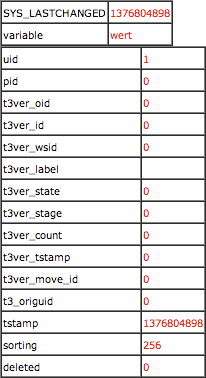
\includegraphics[width=0.6\linewidth]{Images/TypoScript/DebugRegisterAndPage.png}
			\end{figure}
		\end{column}

	\end{columns}

\end{frame}

% ------------------------------------------------------------------------------
% File Links: "register:titleText" and "register:altText"
% ------------------------------------------------------------------------------
% http://forge.typo3.org/issues/44182

\begin{frame}[fragile]
	\frametitle{TSconfig i TypoScript}
	\framesubtitle{Fajl linkovi}

	\begin{itemize}
		\item Fajl linkovi imaju opis, naslov i labelu za alternativni tekst za svaki fajl.
			Moze im se pristupiti preko registara:

			\begin{itemize}
				\item \texttt{register:description}
				\item \texttt{register:titleText}
				\item \texttt{register:altText}
			\end{itemize}

		\item Primer:

			\begin{lstlisting}
				# filelinks
				tt_content.uploads.20 {
				  # link description instead of filename
				  labelStdWrap.data = register:description
				  # output alternative text
				  itemRendering.20.data = register:titleText
				}
			\end{lstlisting}

	\end{itemize}

\end{frame}

% ------------------------------------------------------------------------------
% stdWrap replacement: add optionSplit-support
% ------------------------------------------------------------------------------
% http://forge.typo3.org/issues/42287

\begin{frame}[fragile]
	\frametitle{TSconfig i TypoScript}
	\framesubtitle{stdWrap funkcija: replacement (1)}

	\begin{itemize}
		\item Opcija \texttt{replace} u \texttt{stdWrap}-funkciji \texttt{replacement}\newline
			sada podrzava \texttt{optionSplit}

		\item Primer 1:

			\begin{lstlisting}
				10 = TEXT
				10.value = TYPO3_inspires_people_to_share
				10.replacement.10 {
				  search = _
				  replace = 1 || 2 || 3
				  useOptionSplitReplace = 1
				}
			\end{lstlisting}

			Ishod:\newline
				\texttt{TYPO31inspires2people3to3share}

	\end{itemize}

\end{frame}

% ------------------------------------------------------------------------------
% stdWrap replacement: add optionSplit-support
% ------------------------------------------------------------------------------
% http://forge.typo3.org/issues/42287

\begin{frame}[fragile]
	\frametitle{TSconfig i TypoScript}
	\framesubtitle{stdWrap funkcija: replacement (2)}

	\begin{itemize}
		\item Opcija \texttt{replace} u \texttt{stdWrap}-funkciji \texttt{replacement}\newline
			sada podrzava \texttt{optionSplit}

		\item Primer 2:

			\begin{lstlisting}
				10 = TEXT
				10.value = TYPO3 inspires people to share
				10.replacement.10 {
				  search = #(TYPO3|people|share)#i
				  replace = ${1} CMS || all ${1} || collaborate and ${1}
				  useOptionSplitReplace = 1
				  useRegExp = 1
				}
			\end{lstlisting}

			Ishod:\newline
				\texttt{TYPO3 CMS inspires all people to collaborate and share}

	\end{itemize}

\end{frame}

% ------------------------------------------------------------------------------
% Register values in FilesContentObject
% ------------------------------------------------------------------------------
% http://forge.typo3.org/issues/49480

\begin{frame}[fragile]
	\frametitle{TSconfig i TypoScript}
	\framesubtitle{cObject FILE}

	\begin{itemize}
		\item Dodata su dva registra u cObject FILES:\newline
			\texttt{FILE\_NUM\_CURRENT} i \texttt{FILES\_COUNT}

		\item Primer:

			\lstset{
				basicstyle=\tiny\ttfamily
			}

			\begin{lstlisting}
				10 = FILES
				10 {
				  references {
				    table = tt_news
				    uid.field = uid
				    fieldName = media
				  }
				  renderObj = COA
				  renderObj {
				    10 = TEXT
				    10.value = Renders first file twice
				    10.if.isFalse.data = register:FILE_NUM_CURRENT
				    20 = TEXT
				    20.value = file {register:FILE_NUM_CURRENT} of {register:FILES_COUNT}
				    20.insertData = 1
				  }
				}
			\end{lstlisting}

	\end{itemize}

\end{frame}

% ------------------------------------------------------------------------------
% Category Menu In TypoScript
% ------------------------------------------------------------------------------
% http://forge.typo3.org/issues/51161

\begin{frame}[fragile]
	\frametitle{TSconfig i TypoScript}
	\framesubtitle{Category Menu}

	\begin{itemize}
		\item Generise meni kategorija u TypoScript-u

		\item Primer:

			\lstset{
				basicstyle=\tiny\ttfamily
			}

			\begin{lstlisting}
				page.20 = HMENU
				page.20 {
				  special = categories
				  special {
				    # comma-separated list of categories
				    value = 1
				    # sort by title (stdWrap)
				    sorting = title
				    # sorting "asc" or "desc" (stdWrap)
				    order = desc
				    1 = TMENU
				    1.NO {
				      allWrap = <li> | </li>
				    }
				  }
				}
			\end{lstlisting}

	\end{itemize}

\end{frame}

% ------------------------------------------------------------------------------
% cObject RECORDS with category support
% (slide added in March 2014)
% ------------------------------------------------------------------------------

\begin{frame}[fragile]
	\frametitle{TSconfig i TypoScript}
	\framesubtitle{pristup kategorijama}

	\begin{itemize}
		\item Osobina \texttt{categories} dozvoljava pristup kategorijama\newline
			za cObject RECORDS

		\item Primer:

			\lstset{
				basicstyle=\tiny\ttfamily
			}

			\begin{lstlisting}
				# menu of categorized content elements
				categorized_content = RECORDS
				categorized_content {
				  categories.field = selected_categories
				  categories.relation.field = category_field
				  tables = tt_content
				  conf.tt_content = TEXT
				  conf.tt_content {
				    field = header
				    typolink.parameter = {field:pid}#{field:uid}
				    typolink.parameter.insertData = 1
				    wrap = <li>|</li>
				  }
				  wrap = <ul>|</ul>
				}
			\end{lstlisting}

	\end{itemize}

\end{frame}

% ------------------------------------------------------------------------------
% Category Menu In TypoScript
% ------------------------------------------------------------------------------
% http://forge.typo3.org/issues/51782

\begin{frame}[fragile]
	\frametitle{TSconfig i TypoScript}
	\framesubtitle{CSS i JavaScript fajlovi}

	\begin{itemize}
		\item \texttt{splitChar} se sada moze definisati za \texttt{allWrap} osobine
		\item Wrap sada funkcionise kao standardna \texttt{stdWrap.wrap} metoda
		\item Podrazumevani \texttt{splitChar}-karakter je simbol uspravne crte: \texttt{|}
		\item Ova promena utice na:

			\begin{itemize}
				\item \texttt{includeCSS}
				\item \texttt{includeJSlibs}
				\item \texttt{includeJSFooterlibs}
				\item \texttt{includeJS}
				\item \texttt{includeJSFooter}
			\end{itemize}

	\end{itemize}

\end{frame}

% ------------------------------------------------------------------------------
% Conditions: userFunc Accepts Multiple Arguments
% ------------------------------------------------------------------------------
% http://forge.typo3.org/issues/47159

\begin{frame}[fragile]
	\frametitle{TSconfig i TypoScript}
	\framesubtitle{Uslovi}

	\begin{itemize}
		\item Uslov \texttt{userFunc} sada prihvata vise argumenata

		\item TYPO3 < 6.2
			\begin{lstlisting}
				[userFunc = user_function(argument1)]
			\end{lstlisting}

		\item TYPO3 >= 6.2
			\begin{lstlisting}
				[userFunc = user_function(argument1, argument2, ...)]
			\end{lstlisting}

		\item Primer:
			% \texttt{[userFunc = user\_match(checkSubnet, 192.168)]}

			\lstinline![userFunc = user_match(checkSubnet, 192.168)]!

			\begin{lstlisting}
				function user_match($command, $subnet) {
				  switch($command) {
				    case 'checkSubnet':
				      if (strstr(getenv('REMOTE_ADDR'), $subnet)) { ... }
				  }
				}
			\end{lstlisting}

	\end{itemize}

\end{frame}

% ------------------------------------------------------------------------------
% Conditions: Application Context
% ------------------------------------------------------------------------------
% http://forge.typo3.org/issues/39441
% http://forge.typo3.org/issues/50132

\begin{frame}[fragile]
	\frametitle{TSconfig i TypoScript}
	\framesubtitle{Uslovi}

	\begin{itemize}
		\item Application context se moze odrediti uz pomoc uslova
		\item Wildcards "\texttt{+}" i "\texttt{*}" i regular expressions su podrzani
		\item Primeri:

			\lstset{
				basicstyle=\tiny\ttfamily
			}

			\begin{lstlisting}
				[applicationContext = Development/Debugging, Development/Profiling]
				  # TYPO3 site in development stage
				[global]

				[applicationContext = Production*]
				  # TYPO3 site in production stage
				  # for example "Production/Live" or "Production/Staging"
				[global]

				[applicationContext = /^TestServer\d+$/]
				  # TYPO3 site on TestServer1 or TestServer2 or TestServer3, etc.
				[global]
			\end{lstlisting}

	\end{itemize}

\end{frame}

% ------------------------------------------------------------------------------
% Conditions: IP Supports Keyword devIP
% ------------------------------------------------------------------------------
% http://forge.typo3.org/issues/50092

\begin{frame}[fragile]
	\frametitle{TSconfig i TypoScript}
	\framesubtitle{Uslovi}

	\begin{itemize}

		\item Prilikom koriscenja IP sulova, kljucna rec \texttt{devIP} se moze koristiti kako bi se proverilo da li se IP adresa korisnika podudara sa \texttt{devIpMask} podesavanjima u Install Tool-u
		\item Primer:

%			\lstset{
%				basicstyle=\tiny\ttfamily
%			}

			\begin{lstlisting}
				[IP = devIP]
				  page.10 = TEXT
				  page.10.value = Hello Developer!
				[global]
			\end{lstlisting}

	\end{itemize}

\end{frame}

% ------------------------------------------------------------------------------
% Records Without Default Translation
% ------------------------------------------------------------------------------
% http://forge.typo3.org/issues/24005

\begin{frame}[fragile]
	\frametitle{TSconfig i TypoScript}
	\framesubtitle{Zapisi bez podrazumevanog prevoda}

	\begin{itemize}

		\item Nova opcija \texttt{includeRecordsWithoutDefaultTranslation}
			vraca zapise bez lokalizovanog roditeljskog zapisa\newline
			(ali \texttt{languageField} se podudara sa trenutnim jezikom)

		\item Primer:

			\begin{lstlisting}
				pageContent = CONTENT
				pageContent {
				  table = tt_content
				  select.includeRecordsWithoutDefaultTranslation = 1
				  ...
				}
			\end{lstlisting}

	\end{itemize}

\end{frame}

% ------------------------------------------------------------------------------
% cObject FILES: begin/maxItems options
% ------------------------------------------------------------------------------
% http://forge.typo3.org/issues/52632

\begin{frame}[fragile]
	\frametitle{TSconfig i TypoScript}
	\framesubtitle{cObject FILES}

	\begin{itemize}

		\item cObject FILES sada podrzava \texttt{begin} i \texttt{maxItems} kao osobine

		\item Primer:

			\lstset{
				basicstyle=\tiny\ttfamily
			}

			\begin{lstlisting}
				page.10 = FILES
				page.10 {
				  references {
				    table = pages
				    uid.data = page:uid
				    fieldName = media
				  }

				  # retrieve up to 5 files, beginning at the first (0):
				  begin = 0
				  maxItems = 5

				  renderObj = TEXT
				  renderObj {
				    data = file:current:size
				    wrap = <p>File size:<strong>|</strong></p>
				  }
				}
			\end{lstlisting}

	\end{itemize}

\end{frame}

% ------------------------------------------------------------------------------
% Exclude doktypes From Pagetree
% ------------------------------------------------------------------------------
% http://forge.typo3.org/issues/49279
% http://forge.typo3.org/issues/49356

\begin{frame}[fragile]
	\frametitle{TSconfig i TypoScript}
	\framesubtitle{Iskljuciti doktypes iz stabla sa stranicama}

	\begin{itemize}

		\item Specificni doktypes se mogu iskljuciti iz stabla sa stranicama
		\item Konfigurise se u UserTSconfig (stoga utice na specificnog korisnika ili grupu)
		\item Primeri:

			\begin{lstlisting}
				# exclude "folder" pages
				options.pageTree.excludeDoktypes = 254

				# exclude "folder" and "standard" pages
				options.pageTree.excludeDoktypes = 254,1
			\end{lstlisting}

	\end{itemize}

\end{frame}

% ------------------------------------------------------------------------------
% Hide Modules In Backend
% ------------------------------------------------------------------------------

\begin{frame}[fragile]
	\frametitle{TSconfig i TypoScript}
	\framesubtitle{Sakriti module u administrativnom panelu}

	\begin{itemize}

		\item Moduli se mogu sakriti
		\item Ovo ne utice na pristup modulu\newline
			(koristiti ACL za administratore ili grupe kako bi se zabranio pristup)
		\item Primeri:

			\lstinline!options.hideModules = file, help!
			\lstinline!options.hideModules.web := addToList(func,info)!
			\lstinline!options.hideModules.system = BelogLog!

	\end{itemize}

\end{frame}

% ------------------------------------------------------------------------------
% Alternative Domain For Preview
% ------------------------------------------------------------------------------
% http://forge.typo3.org/issues/30889

\begin{frame}[fragile]
	\frametitle{TSconfig i TypoScript}
	\framesubtitle{Preview Domain}

	\begin{itemize}

		\item Moze se podesiti alternativni domen za pregled stranice/sajta u PageTS
		\item Korisno za sajtove sa vise domena
		\item Primer:

			\lstinline!TCEMAIN.viewDomain = example.com!

	\end{itemize}

\end{frame}

% ------------------------------------------------------------------------------
% Conditions in Backend Layouts
% ------------------------------------------------------------------------------
% http://forge.typo3.org/issues/47588

\begin{frame}[fragile]
	\frametitle{TSconfig i TypoScript}
	\framesubtitle{Uslovi u Backend Layouts}

	\begin{itemize}

		\item Backend layouts sada podrzava uslove
		\item Primer:

			\lstset{
				basicstyle=\tiny\ttfamily
			}

			\begin{lstlisting}
				backend_layout {
				  colCount = 2
				  rowCount = 1
				  rows {
				    1 {
				      columns {
				        1.name = Main
				        1.colPos = 0
				        2.name = Right
				        2.colPos = 1
				      }
				    }
				  }
				}

				[PIDupinRootline = 123]
				  # remove right column in branch of page ID 123
				  backend_layout.rows.1.columns.2 >
				[global]
			\end{lstlisting}

	\end{itemize}

\end{frame}

% ------------------------------------------------------------------------------
% Miscellaneous
% ------------------------------------------------------------------------------
% http://forge.typo3.org/issues/34597 (showForgotPassword)
% http://forge.typo3.org/issues/50138 (showForgotPassword)
%
% http://forge.typo3.org/issues/19732 (Content-Length)
%
% http://forge.typo3.org/issues/16386 (Indexed Search) - wow: submitted 7 years ago :-)

\begin{frame}[fragile]
	\frametitle{TSconfig i TypoScript}
	\framesubtitle{Razno}

	\begin{itemize}

		\item Omoguciti/onemoguciti "forgot password" link uz pomoc opcije \small\texttt{showForgotPassword}\normalsize\newline
			(korisno ukoliko je ukljuceno vise login formi preko EXT:felogin na jednoj strani)

		\item HTTP response je sada ukljucen u zaglavlje \texttt{Content-length}

			\begin{itemize}
				\item Ubrzava renderovanje ukoliko je pipelining omogucen u Apache-u
				\item moze se konfigurisati kroz \texttt{config.enableContentLengthHeader}
			\end{itemize}

		\item Result lista EXT:indexed\_search ima \texttt{stdWrap}-properties\newline
			(opcija: \texttt{plugin.tx\_indexedsearch.resultlist\_stdWrap})

	\end{itemize}

\end{frame}

% ------------------------------------------------------------------------------

